\documentclass[a4paper,12pt,fleqn]{article}%fleqn pour aligner les equations à gauche
\usepackage{../../Styles/Exercice}

\newcommand{\chnum}{Chapitre 6}
\newcommand{\chtitle}{Le son}
\newcommand{\dtype}{Exercices}

\begin{document}
\maketitle
\begin{multicols}{2}
\section{Le diapason}
Le diapason est un outil utilisé par les musiciens pour s'accorder. En effet, s'il est parfaitement dimensionné, la vibration de la partie métallique permet la production d'un son de fréquence $f$, utilisé pour l'accordage des instruments.\\
\textbf{Questions :}
\begin{enumerate}
	\item Justifier que le son associé au signal ci-après est un son pur.
	\item Déterminer la durée $\Delta t$ de quatre périodes du signal. Déduisez la période $T$ du signal.
	\item Calculer la fréquence $f$ du son produit par un diapason.
\end{enumerate}
\noindent 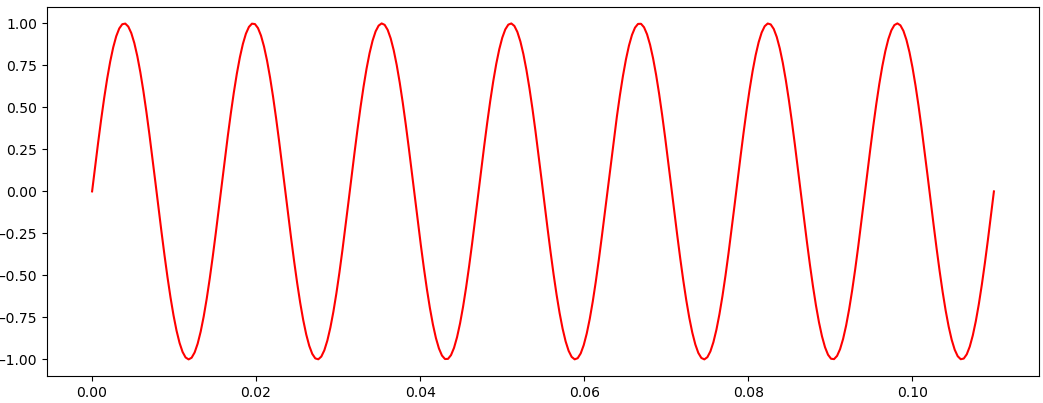
\includegraphics[width=1\linewidth]{1ES_C6_Exercices_Fig1.png}
	
\section{Le violon}
Le violon est un instrument à cordes frottées. À l'aide d'un archet, le musicien exerce une excitation sur une corde qui permet de la faire vibrer. En fonction de la position des doigts sur le manche, le violoniste peut modifier la note de la corde en raccourcissant la longueur $l$. Les autres caractéristiques de la corde restent inchangées.\\
On propose dans cet exercice de déterminer la longueur optimale $l$ des cordes d'un violon pour un passage le plus aisé possible entre les notes (c’est à dire dans avoir à déplacer la main le long du manche). La troisième corde, accordée à vide pour obtenir un \textit{la3}, doit présenter un écartement entre l’index (pour obtenir un \textit{la\#3}) et l’auriculaire (pour obtenir un \textit{mi4}), techniquement réalisable sans avoir à bouger la main.\\
On note $l_1$ et $f_1$ la longueur et la fréquence fondamentale de la corde associées à l’obtention du \textit{la\#3} ; $l_2$ et $f_2$ les même grandeurs associées à l’obtention du \textit{mi4}.\\
\begin{tabular}{|>{\centering}m{.25\linewidth}|>{\centering}m{.15\linewidth}|>{\centering}m{.15\linewidth}|>{\centering\arraybackslash}m{.15\linewidth}|}
	\hline
	\textbf{Note} & \textit{la3} & \textit{la\#3} & \textit{mi4}\\
	\hline
	\textbf{Fréquence (\unit{\hertz})} & \num{440,00} & \num{446,16} & \num{659,26}\\
	\hline
\end{tabular}
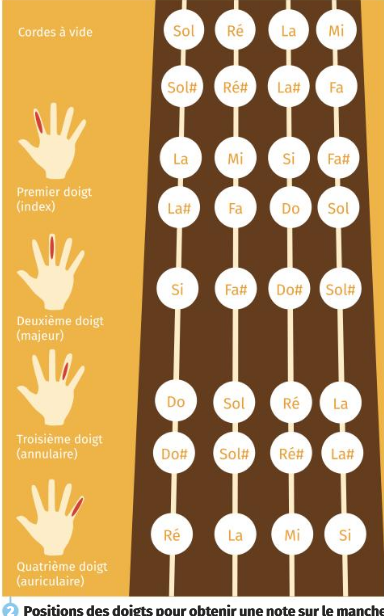
\includegraphics[width=\linewidth]{1ES_C6_Exercices_Fig2.png}

\textbf{Questions :}
\begin{enumerate}
	\item Estimer l'écartement maxiaml possible, noté $e$ et exprimé en centimètres (\unit{\centi\meter}), entre votre index et votre auriculaire.
	\item Sachant que la fréquence fondamentale d'une corde vibrante est inversement proportionnelle à sa longueur, démontrer que $f_1 \cdot l_1 = f_2 \cdot l_2$.
	\item En précidant dans un premier temps la relation entre $l_1$, $l_2$ et $e$, déterminer l'expression de la longueur $l_2$ en fonction de $f_1$, $e$ et $f_2$.
	\item En réutilisant le résultat de la question 2 pour le \textit{la3} et le \textit{mi4}, démontrer que la longueur $l$ des cordes s'exprime $l=\dfrac{f_2 \cdot f_1 \cdot e}{f \cdot (f_2-f_1)}$ et calculer cette longueur pour l'écartement $e$ estimé à partir de vos doigts. Ce résultat est-il cohérent avec la dimension d'un violon traditionnel ?
\end{enumerate}

\section{L'accordage d'une guitare}
L’accordage d’un instrument est un impératif pour tous les musiciens. Si celui-ci se révèle plus simple avec les nouvelles technologies (accordeur électronique, application sur smartphone), il n’en demeure pas moins qu’il est nécessaire pour un bon musicien de savoir s’accorder à l’oreille.\\
Tour les musiciens ne sont pas capables de reconnaître une fréquence fondamentale à sa seule écoute. Pour autant, en connaissant quelques règles sur les fréquences fondamentales des sons produits par la vibration des cordes, on peut facilement accorder les cordes d’une guitare entre elles pour obtenir un son mélodieux.\\
A chaque fois que l’on appuie sur une corde de la guitare, on diminue la longueur de la partie vibrante. Comme le manche est pourvu d’un certain nombre de frettes (barres métalliques perpendiculaires à l’axe du manche), les fréquences possibles sont quantifiées, c’est à dire qu’il n’est pas possible d’obtenir n’importe quelle fréquence, mais des fréquences définies par la distance entre le chevalet et les frettes. Ces distances $l_n$ évoluent de la manière suivante en fonction de $l$, la longueur de la corde et $n$ un entier naturel correspondant au numéro de la frette : $$l_n = \dfrac{l}{2^{\dfrac{n}{12}}}$$
Or, pour accorder deux cordes consécutives sur la guitare, il suffit d’appuyer sur la corde de fréquence la plus basse au niveau de l’une de ses frettes et d’accorder la seconde pour atteindre la même fréquence.

\begin{figure}[h!]
	\begin{minipage}{.48\linewidth}
		\centering
		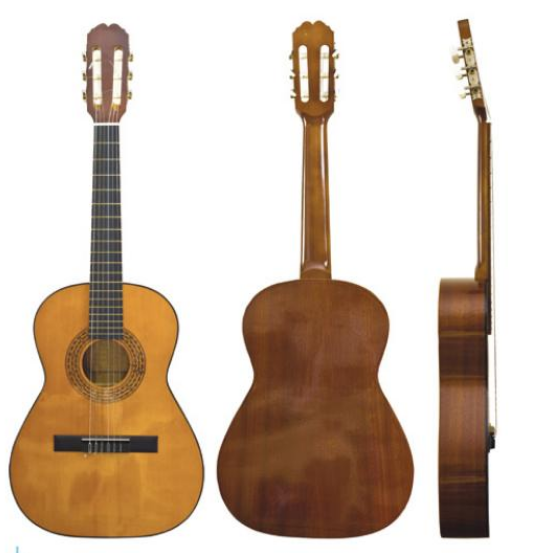
\includegraphics[width=\linewidth]{1ES_C6_Exercices_Fig3.png}
	\end{minipage}\hspace{1em}
	\begin{minipage}{.48\linewidth}
		\centering
		\begin{tabular}{|c|c|}
			\textbf{Numéro de la corde (de gauche à droite sur la photographie)} & \textbf{Fréquence fondamentale à obtenir pour un bon accordage (\unit{\hertz})}\\
			\hline
			\num{1} & \num{82,41}\\
			\hline
			\num{2} & \num{110,00}\\
			\hline
			\num{3} & \num{146,83}\\
			\hline
			\num{4} & \num{196,00}\\
			\hline
			\num{5} & \num{246,94}\\
			\hline
			\num{6} & \num{329,63}\\
		\end{tabular}
		\caption*{Fréquence fondamentale à obtenir pour chaque corde de la guitare}
	\end{minipage}
\end{figure}
\textbf{Questions :}
\begin{enumerate}
	\item Préciser comment évolue la fréquence fondamentale du son émis par une corde vibrante dont on diminue la longueur. Comment peut-on exprimer mathématiquement cette relation ?
	\item Exprimer al longueur de la corde $l_n$ entre la frette en contact et le chevalet, en fonction de la fréquence fondamentale émise notée $f'$, la fréquence fondamentale $f$ de la corde à vide et $l$ la longueur de la corde à vide.
	\item Démontrer que $\dfrac{f}{f'} = \dfrac{1}{2^{\dfrac{n}{12}}}$. On admet par la suite que $n = \dfrac{12}{Log(2)}\cdot Log (\frac{f'}{f})$
	\item Calculer chaque numéro de frette $n$ sur laquelle il est nécessaire de poser son doigt pour pouvoir augmenter la fréquence fondamentale du son produit par la corde de façon à obtenir la même fréquence fondamentale que la corde suivante.
\end{enumerate}

\section{Concert}
Je me situe dans une salle de concert au premier rang, à \SI{5}{m} de la scène. le niveau d'intensité sonore que je preçois vaut \SI{105}{dB}. Lorsque je m'éloigne de \SI{15}{m}, quelle est le niveau d'intensité sonore que je perçois alors ?
\end{multicols}
\end{document}